% !TeX spellcheck = en_US
% !TeX root = ../main.tex
\section{Results}
\label{sec:results}

In the following, we apply the framework presented in Section~\ref{sec:methods} to the data introduced in Section~\ref{subsec:data:instance}, i.e., codified law comprising federal statutes and regulations in the United States and Germany over the $22$ years from $1998$ to $2019$ (inclusive).
We start by examining the growth of the United States and German national legal systems (henceforth: the national legal systems) as viewed through the lens of our data (Section~\ref{subsec:results:growth}).
Next, we investigate the macro-level, meso-level, and micro-level connectivity of these national legal systems (Section~\ref{subsec:results:connectivity}).
Finally, we explore the evolution of selected chapters of the USC and the CFR and selected German statutes and regulations within their national legal systems in a case study focusing on financial regulation (Section~\ref{subsec:results:profiles}).
The results we report are mostly descriptive, and as discussed in Section~\ref{sec:discussion}, identifying causal factors behind the dynamics we observe or interpreting our results using a qualitative approach is left to future research.

\vspace*{30pt}
\subsection{Growth}
\label{subsec:results:growth}

Figure \ref{fig:basic-statistics} summarizes the growth of the United States legal system and the German legal system as measured by the tokens, structural elements, and lateral references contained in their codified law. 
Each row of the figure corresponds to a country, and each column corresponds to a document type. 
All counts are divided by their value in $1998$, i.e., Figure~\ref{fig:basic-statistics} depicts growth relative to the $1998$ baseline.
Supplementing the time series data, 
Table~\ref{tab:basic-statistics} provides the absolute counts for $1998$ and $2019$ and the total percentage change between these years ($\Delta$).

\begin{figure}
	\centering
	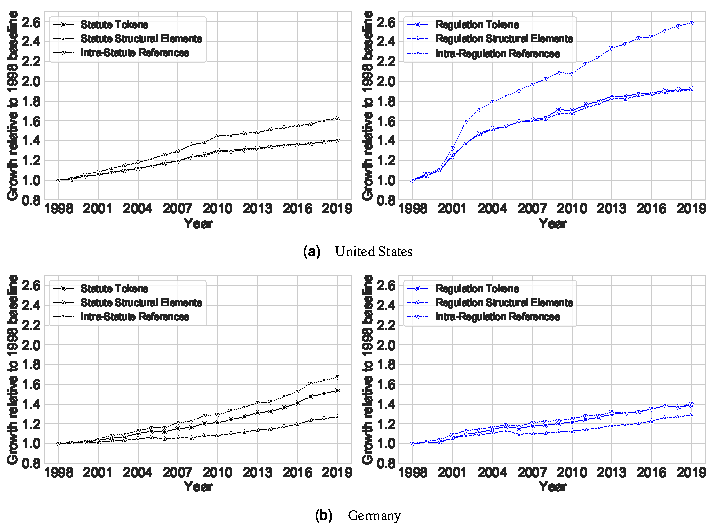
\includegraphics[width=\textwidth]{figure_5}
	\caption{Growth relative to the $1998$ baseline for statutes (left) and regulations (right) in the United States (top) and Germany (bottom).}\label{fig:basic-statistics}
\end{figure}

\begin{table}
	\centering
	% !TeX spellcheck = en_US
			\renewcommand{\arraystretch}{1.5}
				\begin{tabular}{lrrrrrr}
\toprule & \multicolumn{3}{c}{\textbf{Statutes}} & \multicolumn{3}{c}{\textbf{Regulations}} \\
            & 1998   & 2019   &   $\Delta$ & 1998   & 2019   &   $\Delta$ \\
\midrule
 \textbf{Tokens}     & 15.2~M               & 21.4~M               &                      41 & 43.9~M                  & 84.3~M                  &                         92 \\
 \textbf{Structures} & 516.2~K              & 838.8~K              &                      63 & 1.4~M                   & 2.7~M                   &                         91 \\
 \textbf{References} & 80.1~K               & 112.1~K              &                      40 & 134.6~K                 & 348.4~K                 &                        159 \\
\bottomrule
\end{tabular}
				
				{\vspace*{6pt}\small \textbf{\textsf{(a)}}\quad United States}\vspace*{12pt}
			
				\begin{tabular}{lrrrrrr}
\toprule & \multicolumn{3}{c}{\textbf{Statutes}} & \multicolumn{3}{c}{\textbf{Regulations}} \\
            & 1998   & 2019   &   $\Delta$ & 1998   & 2019   &   $\Delta$ \\
\midrule
 \textbf{Tokens}     & 5.0~M                & 7.7~M                &                      54 & 3.9~M                   & 5.4~M                   &                         39 \\
 \textbf{Structures} & 130.6~K              & 166.0~K              &                      27 & 87.9~K                  & 113.7~K                 &                         29 \\
 \textbf{References} & 86.4~K               & 144.6~K              &                      67 & 33.5~K                  & 47.1~K                  &                         41 \\
\bottomrule
\end{tabular}
				
				{\vspace*{6pt}\small \textbf{\textsf{(b)}}\quad Germany} 

	\caption{(Rounded) size of the national legal systems of the United States (top) and Germany (bottom) as measured by the tokens, structural elements, and references in their codified law in $1998$ and $2019$, including the total percentage change between these years ($\Delta$).}\label{tab:basic-statistics}
\end{table}

Figure~\ref{fig:basic-statistics} and Table~\ref{tab:basic-statistics} show that over the last two decades, the legal systems of both countries have grown substantially.  
In the United States, the USC (containing codified statutes) has over $60$ new structural elements (e.g., chapters, parts, or sections) in $2019$ for every $100$ such elements it had in $1998$.
Notably, as evident from the upper left panel of Figure~\ref{fig:basic-statistics}, the growth rate of the USC appears to have experienced two distinct periods when measured by its structural elements: 
one period with a monotonic growth rate of approximately $4~\%$ per year ($1998$--$2010$), followed by another period with a decelerated monotonic growth rate of approximately $2~\%$ per year ($2010$--$2019$). 
At a slightly lower level, this trend also occurs for both the number of tokens and the number of intra-USC references. 
For example, there are approximately $40$ new tokens or references in $2019$ for every $100$ tokens or references that existed in $1998$.
Shifting the focus for the United States to the CFR (containing codified regulations), as observable from the upper right panel of Figure~\ref{fig:basic-statistics}, the quantity of regulations has increased by an even greater factor.  
For every $100$ structural elements or tokens that were present in $1998$, approximately $90$ additional elements or tokens exist in $2019$. 
This increase is even more extreme for intra-CFR references, where there are almost $160$ \emph{new} references in $2019$ for every $100$ that existed in $1998$.  
Apart from brief intervals of stagnation or slight decrease ($2009$--$2010$, $2013$--$2014$), 
these increases have been monotonic.

Corresponding trends for German statutes and regulations are presented in the bottom row of Figure \ref{fig:basic-statistics}.  
Growth in the German legal system has been qualitatively similar to that in the United States legal system but quantitatively less pronounced and of different functional shape. 
For both German statutes and German regulations, there are approximately $30$ new structural elements in $2019$ for every $100$ that existed in $1998$. 
Unlike in the United States, however, this growth has been non-monotonic: 
When measured through structural elements, both statutes and regulations experienced some periods of shallow decline between $2005$ and $2010$.
These shrinking periods are generally not mirrored by the token and lateral reference counts, with one notable exception:
In the period from $2005$ to $2006$, \emph{all} German statistics decreased. 
This is likely due to statutes aiming to cleanse the law (\emph{Rechtsbereinigungsgesetze}), eight of which were introduced in $2006$ (recall that our $2006$ snapshot represents the law at the \emph{end} of $2006$).\footnote{%
These statutes are: 
(1) Erstes Gesetz über die Bereinigung von Bundesrecht im Zuständigkeitsbereich des Bundesministeriums des Innern vom 19. Februar 2006 (BGBl.~I~S.~334),
(2) Gesetz zur Bereinigung des Bundesrechts im Zuständigkeitsbereich des Bundesministeriums für Ernährung, Landwirtschaft und Verbraucherschutz vom 13. April 2006 (BGBl.~I~S.~855),
(3) Erstes Gesetz über die Bereinigung von Bundesrecht im Zuständigkeitsbereich des Bundesministeriums der Justiz vom 19. April 2006 (BGBl.~I~S.~866),
(4) Erstes Gesetz zur Bereinigung des Bundesrechts im Zuständigkeitsbereich des Bundesministeriums für Wirtschaft und Technologie und im Zuständigkeitsbereich des Bundesministeriums für Arbeit und Soziales vom 19. April 2006 (BGBl.~I~S.~894),
(5) Gesetz zur Änderung und Bereinigung des Lastenausgleichsrechts vom 21. Juni 2006 (BGBl.~I~S.~1323),
(6) Gesetz über die Bereinigung von Bundesrecht im Zuständigkeitsbereich des Bundesministeriums für Arbeit und Soziales und des Bundesministeriums für Gesundheit vom 14. August 2006 (BGBl.~I~S.~1869),
(7) Erstes Gesetz über die Bereinigung von Bundesrecht im Zuständigkeitsbereich des Bundesministeriums für Verkehr, Bau und Stadtentwicklung vom 19. September 2006 (BGBl.~I~S.~2146), and
(8) Zweites Gesetz über die Bereinigung von Bundesrecht im Zuständigkeitsbereich des Bundesministeriums des Innern vom 2. Dezember 2006 (BGBl.~I~S.~2674).
}
In total, there are approximately $55$ new statute tokens in Germany in $2019$ for every $100$ such tokens that existed in $1998$. 
Like \emph{regulations} in the United States, German \emph{statutes} experienced a greater increase in the quantity of lateral references than in other metrics: 
For every $100$ references in $1998$, there are approximately $70$ new references in $2019$. 
For German \emph{regulations}, as for \emph{statutes} in the United States, the rate of change has been more similar across metrics, with growth varying roughly between $30~\%$ and $40~\%$ (as noted in Table~\ref{tab:basic-statistics}).
At a high level, the growth of the German legal system thus seems to be driven by statutes, whereas the growth of the United States legal system appears to be driven by regulations.

\begin{figure}
	\centering
	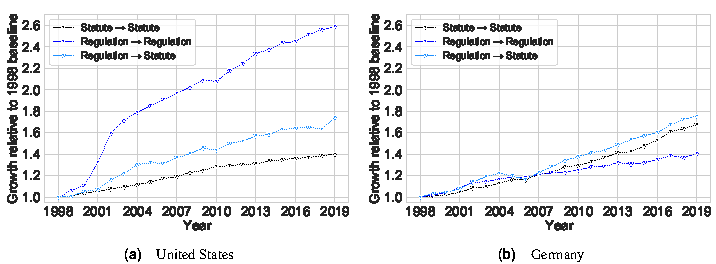
\includegraphics[width=\textwidth]{figure_6}
	\caption{Growth relative to the $1998$ baseline for lateral and upward references in the United States (left) and Germany (right).}\label{fig:crossref-evolution}
\end{figure}

Figure~\ref{fig:basic-statistics} and Table~\ref{tab:basic-statistics} only account for \emph{lateral} references, excluding references between documents of different types. 
Therefore, Figure~\ref{fig:crossref-evolution} shows growth relative to the $1998$ baseline for lateral and \emph{upward} (i.e., regulation-to-statute) references. 
We exclude \emph{downward} references because they are very few in number (which means that even a small absolute increase results in a large relative increase) 
but note that, contrary to the legal theory intuition, they \emph{do} occur.\footnote{%
The total number of downward references in the United States increases from $24$ in $1998$ to $90$ in $2019$.
In Germany, it rises from $305$ to $833$.
}
As evident from Figure~\ref{fig:crossref-evolution}, upward references have grown at similar rates in both countries, with approximately $80$ new upward references existing in $2019$ for every $100$ upward references that existed in $1998$. 
This relative increase is larger than that of the lateral references in both countries, with the exception of lateral regulation references in the United States, whose growth rate dwarfs all others. 
Since the token and structural element growth rates of German regulations are lower than or similar to those of German statutes, this means that over the period under study, connectivity between statutes and regulations in Germany has grown faster than connectivity within statutes or within regulations. 

To evaluate how the growth in the number of references affects the differences in the prominence of individual sections of codified law in the legal systems under study, in Figure~\ref{fig:degree-distribution}, we examine the in-degree distribution and the out-degree distribution of the graphs induced by the reference edges in $1998$ and $2019$ (an analogous figure normalizing section degrees by section size in tokens can be found in Section~4.1 of the \thesi).  
Since these distributions are highly skewed (as in many graphs arising from complex systems), we plot them on a log-log scale. 

\begin{figure}
	\centering
	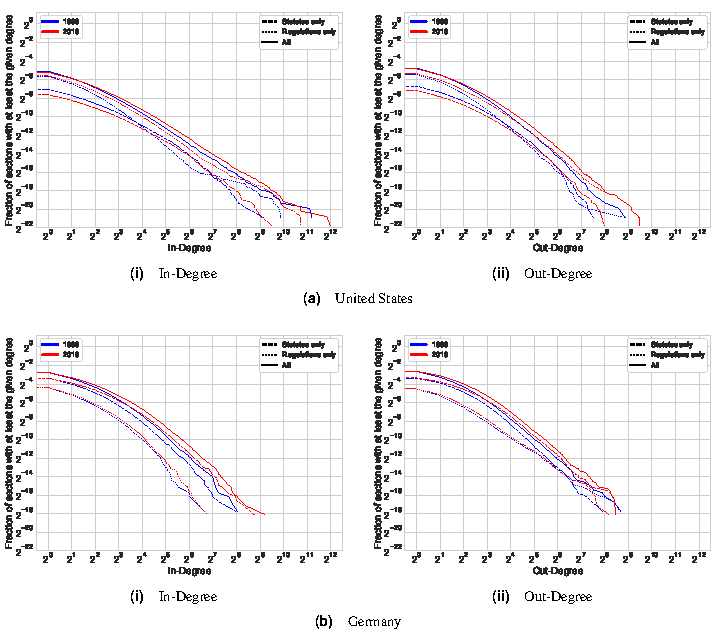
\includegraphics[width=\textwidth]{figure_7}
	\caption{In-degree (left) and out-degree (right) distributions for the United States (top) and Germany (bottom) in $1998$ (blue) and $2019$ (red) when considering statutes only (dashed line), regulations only (dotted line), or statutes and regulations (solid line).}\label{fig:degree-distribution}
\end{figure}

All distributions plotted in Figure~\ref{fig:degree-distribution} demonstrate features common among graphs arising from bibliometric dynamics. 
For example, most sections of statutes and regulations in the United States and Germany are referenced very few times (if at all). 
The detailed characteristics of the distributions, however, differ between distribution types, document types, and countries:
For the United States, the out-degree distributions exhibit less right skew than their in-degree counterparts, 
while in Germany, we observe the opposite: 
All out-degree distributions are either within an order of magnitude of or have a longer and thicker right tail than their in-degree counterparts. 
Similarly, the sections contained in United States regulations exhibit a higher degree of skew in their in-degree distributions than the sections contained in United States statutes 
(e.g., a higher fraction of these sections has more than $500$ ingoing references), 
but in Germany, the opposite phenomenon occurs at a lower absolute level: 
There are many statute sections with more than $100$ ingoing references but hardly any regulation sections clearing that threshold. 
These national divergences might be partly due to the differing ratio between statutes and regulations, but they could also point to peculiarities in United States and German drafting style.

Comparing \emph{all} distributions across countries, we observe that the United States legal system exhibits more extreme statistics than the German legal system (which might, at least in part, be due to its larger size).
Finally, we see that from $1998$ to $2019$, most distributions shift to the right, i.e., the tails become both longer and thicker, 
which is in line with bibliometric preferential attachment dynamics \cite{merton1968,price1976}.
This indicates that reference growth has disparate impact, amplifying the differences in relevance between the individual sections contained in United States and German statutes and regulations.
As a consequence, the difficulty of navigating the law increases more slowly than the growth of the reference count may suggest. 

\vspace*{12pt}
\subsection{Connectivity}
\label{subsec:results:connectivity}

When exploring the connectivity of the national legal systems of the United States and Germany over time, we distinguish between the macro level, the meso level, and the micro level as suggested in Section~\ref{subsec:methods:connectivity}.

\vspace*{6pt}
\subsubsection{Macro-level connectivity}
\label{subsubsec:results:connectivity:macro}

To understand how the United States legal system and its German counterpart organize and process information, we investigate the connectivity of the graphs containing code sections as nodes and references between them as edges. 
Figure~\ref{fig:connectivity-components} displays the number of non-trivial (weakly) connected components (i.e., components with more than one node) in these graphs over time, 
in absolute terms and per $1000$ tokens.
It shows that the connectivity in the graphs containing only statute sections is generally higher than that in the graphs containing only regulation sections or sections of both document types.
Furthermore, while the United States system seems more fragmented than the German system (Figure~\ref{fig:connectivity-components}~(a)) when considering absolute numbers, it turns out to be relatively less fragmented when normalizing for system size (Figure~\ref{fig:connectivity-components}~(b)).

\begin{figure}
	\centering
	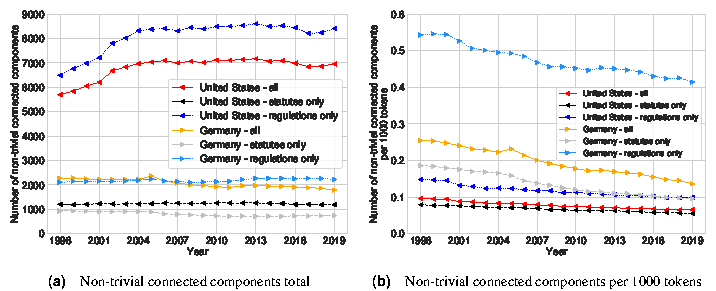
\includegraphics[width=\textwidth]{figure_8}
	\caption{Development of reference connectivity as measured by the absolute number of non-trivial (weakly) connected components (left) and the number of non-trivial (weakly) connected components per $1000$ tokens (right) in the graphs induced by reference edges between all sections (solid lines), statute sections only (dashed lines), and regulation sections only (dotted lines) in the United States (left-pointing triangles) and Germany (right-pointing triangles).}\label{fig:connectivity-components}
\end{figure}

For a more granular connectivity assessment over time, Figure~\ref{fig:connectivity-all} shows, for each year from $1998$ to $2019$, what fraction of statute sections and regulation sections in each country is contained in the largest connected component, satellite components, or isolates, 
and how the largest connected component is composed internally. 
The underlying graphs do not distinguish between sections of different document types; 
analogous figures considering statute sections only and regulation sections only can be found in Section~4.2 of the \thesi.
In both the United States and Germany, the largest connected component is growing as the fraction of sections contained in both satellites and singletons decreases, 
and the difference between the largest connected component fraction in $1998$ and that in $2019$ is around $10~\%$. 
However, the relative size of these largest connected components varies substantially between the two countries: 
In the United States, the largest connected component has grown from about $40~\%$ to nearly $50~\%$, 
while in Germany, its size has increased from circa $55~\%$ to roughly $65~\%$.
Furthermore, the fraction of isolates (sections that neither reference another section nor get referenced by another section) is larger in the United States (around $45~\%$ in $2019$) than in Germany (below $30~\%$ in $2019$).

\begin{figure}
	\centering
	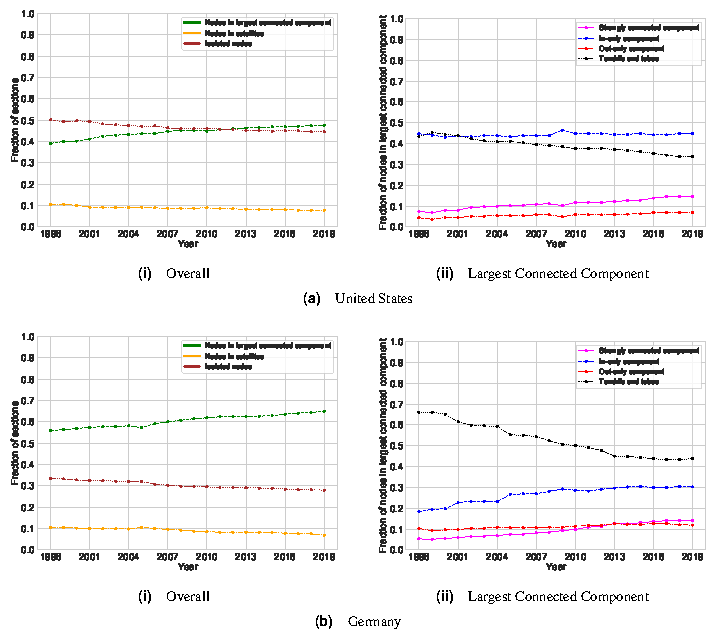
\includegraphics[width=\textwidth]{figure_9}
	\caption{Development of reference connectivity in the United States (top) and Germany (bottom) as measured by the fraction of sections contained in the largest connected component (left), along with the internal structure of that component (right).}\label{fig:connectivity-all}
\end{figure}

When focusing on the largest connected component and taking edge directions into account, the differences between the two countries become even more pronounced.  
In the United States, the fraction of the largest connected component contained in the in-only component is almost equal to that contained in its tendrils and tubes in $1998$, and both lie around $45~\%$.
Over time, these fractions diverge as the strongly connected component and the out-only component grow and the in-only component stagnates. 
In Germany, however, tendrils and tubes dominate in $1998$, accounting for more than $65~\%$ of nodes, 
but by $2019$, their fraction has declined to less than $45~\%$, while the strongly connected component and the out-only component have grown at low levels and the in-only component has gained more than $50~\%$ in fractional size (growing from less than $20~\%$ to over $30~\%$).

Notably, in both legal systems, the out-only component accounts for the smallest fraction of sections in $2019$ (around $7~\%$ in the United States and around $12~\%$ in Germany), followed by the strongly connected component, with none of them containing more than $15~\%$ of all sections, while the in-component is twice as large in Germany and thrice as large in the United States.
Hence, at least when considering code sections as nodes and references between them as edges, both national legal systems do not exhibit the bowtie structure observed in biological systems (small strongly connected component with larger in-only and out-only components \cite{friedlander2015}) or that found in early measurements of the World Wide Web (all components, including tendrils and tubes, of roughly the same size, with a slightly larger strongly connected component \cite{broder2000}).
Rather, the legal systems we study are shaped more like rockets, with the in-only component as their base, tendrils and tubes as their fins, the strongly connected component as their body, and the out-component as their nose cone (see Figure~\ref{fig:rocket} for an illustration).
The rocket structure mirrors both the hierarchical structure of legal systems (large in-only component, small out-only component) and the fact that some areas of law function relatively independently (many tendrils and tubes; also evident from the nontrivial fraction of nodes outside the largest connected component). 
This suggests that it might be characteristic of legal systems in general, but more research is needed to corroborate this hypothesis.
Similarly, it would be interesting to investigate how our observations change if we include, e.g., non-atomic references (which, by definition, interconnect multiple sections).

\begin{figure}[h]
	\centering
	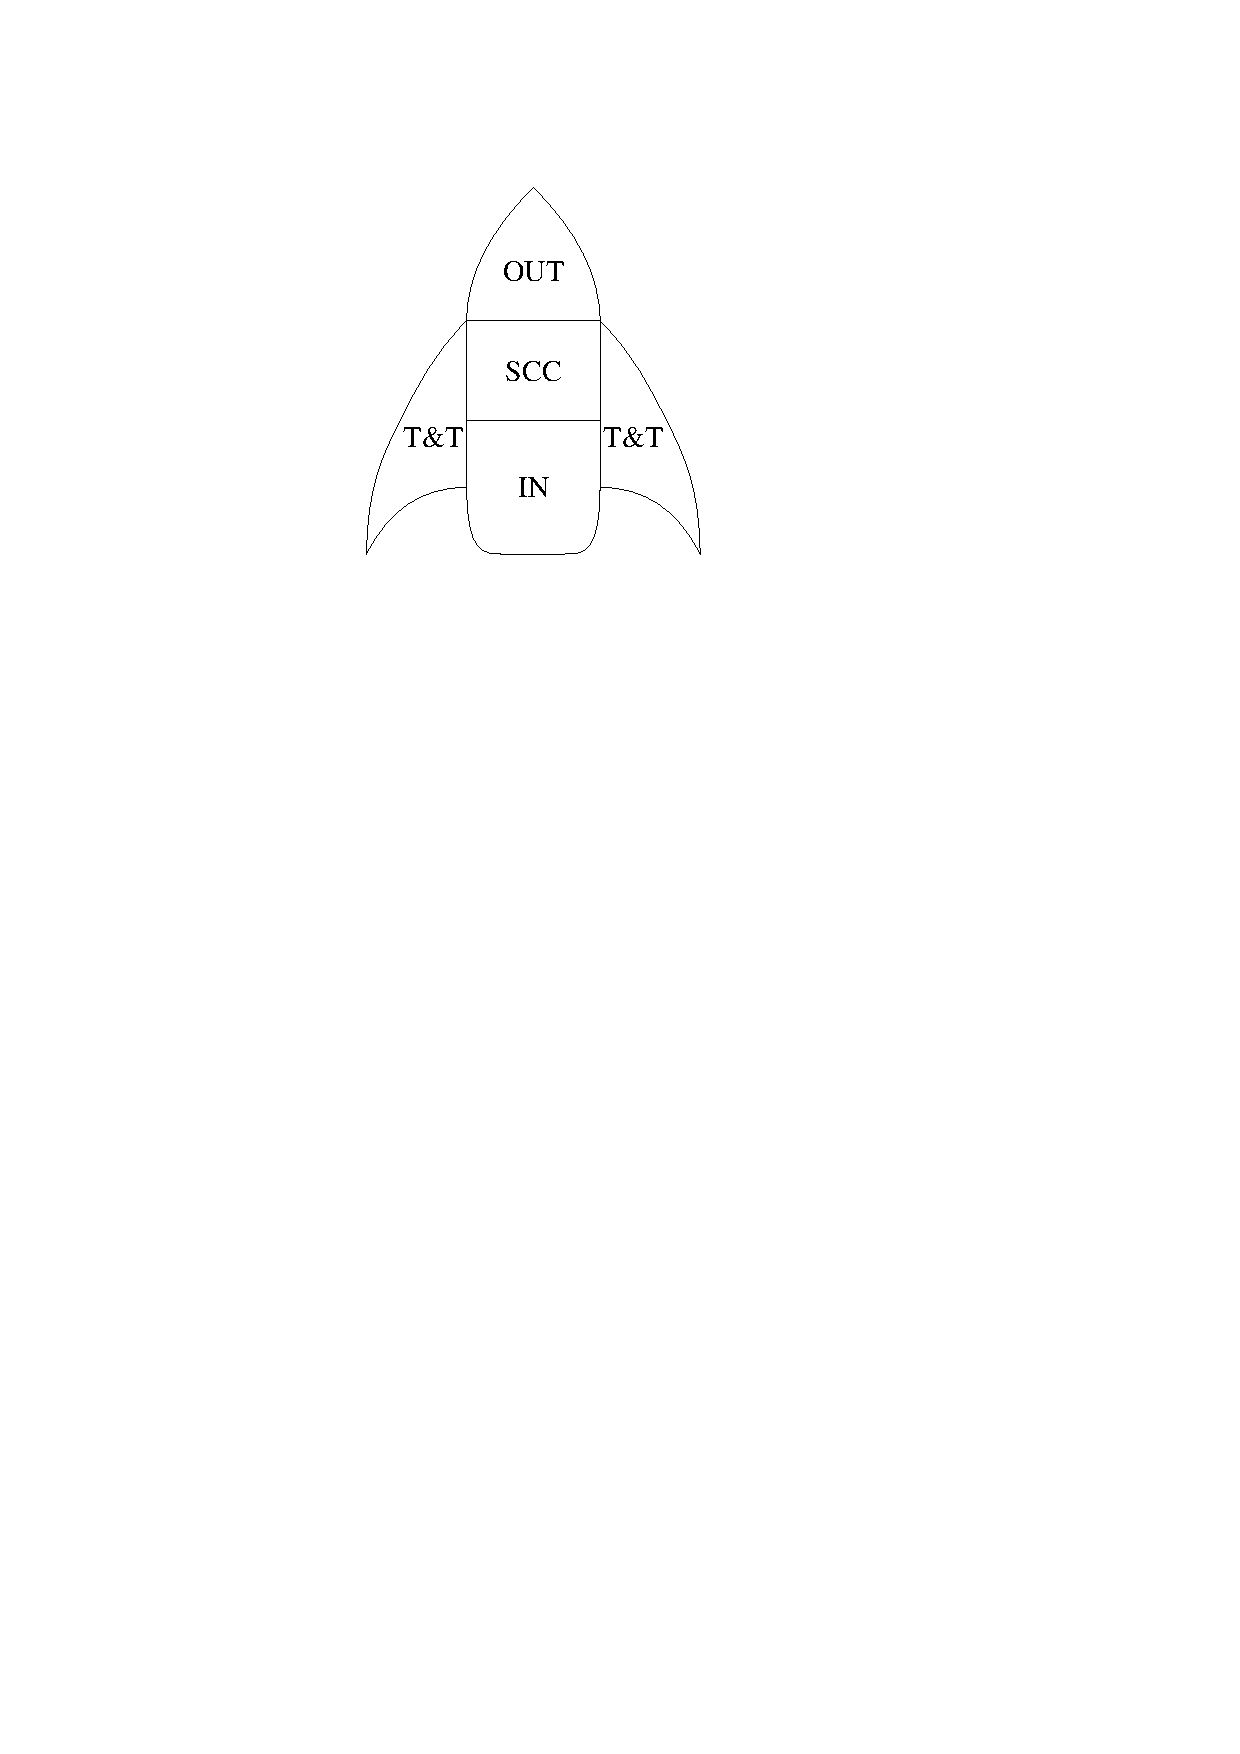
\includegraphics{figure_10}
	\caption{Rocket structure of a legal system when viewed through the lens of macro-level connectivity, with the in-component (IN) as the rocket's base, the strongly connected component (SCC) as the body, the out-component (OUT) as the nose cone, and tendrils and tubes (T\&T) as the fins.}\label{fig:rocket}
\end{figure}

\vspace*{12pt}
\subsubsection{Meso-level connectivity}
\label{subsubsec:results:connectivity:meso}

When analyzing the connectivity of the United States and German legal systems at the meso level, our goal is to create a dynamic, data-driven map of their codified law.
To this end, for both the United States and Germany, we compute cluster families as described in Section~\ref{subsubsec:methods:connectivity:meso}, 
using quotient graphs on the chapter level in the United States and on the statute or regulation level (or the book level, if available) in Germany. 
Here, we choose $100$ as the preferred number of \emph{Infomap} clusters and $15~\%$ of tokens as the edge threshold for constructing the cluster family graph (for details on how we handle text that does not lie in a chapter as well as a sensitivity analysis of the parameter choice, see Sections~4.3.1 and~4.3.4 of the \thesi). 
We calculate how many tokens from statutes and regulations these families contain in each year from $1998$ to $2019$.
By construction, our cluster families unite sets of related rules that can be thought of as different areas of law, where---unlike in, e.g., the title structure of the USC or the German finding aids' subject classification (Fundstellennachweise, FNA)---the categorization is based solely on the empirically observed reference relationships between the legal documents in our data.

Figure~\ref{fig:families} shows the evolution ($1998$--$2019$) of the ten cluster families with the largest number of tokens in $2019$ (henceforth: top ten cluster families) for each country, which we label leveraging our subject matter expertise (details on the labeling procedure and complementary linguistic statistics can be found in Section~4.3.2 of the \thesi).
Most families either represent a traditional field of law (e.g., property law or financial regulation) or concern a real-life domain (e.g., energy or vocational training).
A few families hold clusters from more diverse backgrounds and are therefore hard to interpret at first sight (e.g., a family containing military, public finance, and research regulation in the United States or a family containing court procedure, data security, and telecommunications in Germany).
However, a more detailed examination of the individual clusters constituting these families uncovers nuanced underlying topics (e.g., grants and commercial activity by the federal government in the example from the United States, and data protection in public [including court] proceedings in the example from Germany).
Hence, in summary, the method sketched in Section~\ref{subsubsec:methods:connectivity:meso} produces an informative map of the codified law for both countries we investigate (at the resolution level determined by our parametrization).

\begin{figure}
	\centering
	\vspace*{-9pt}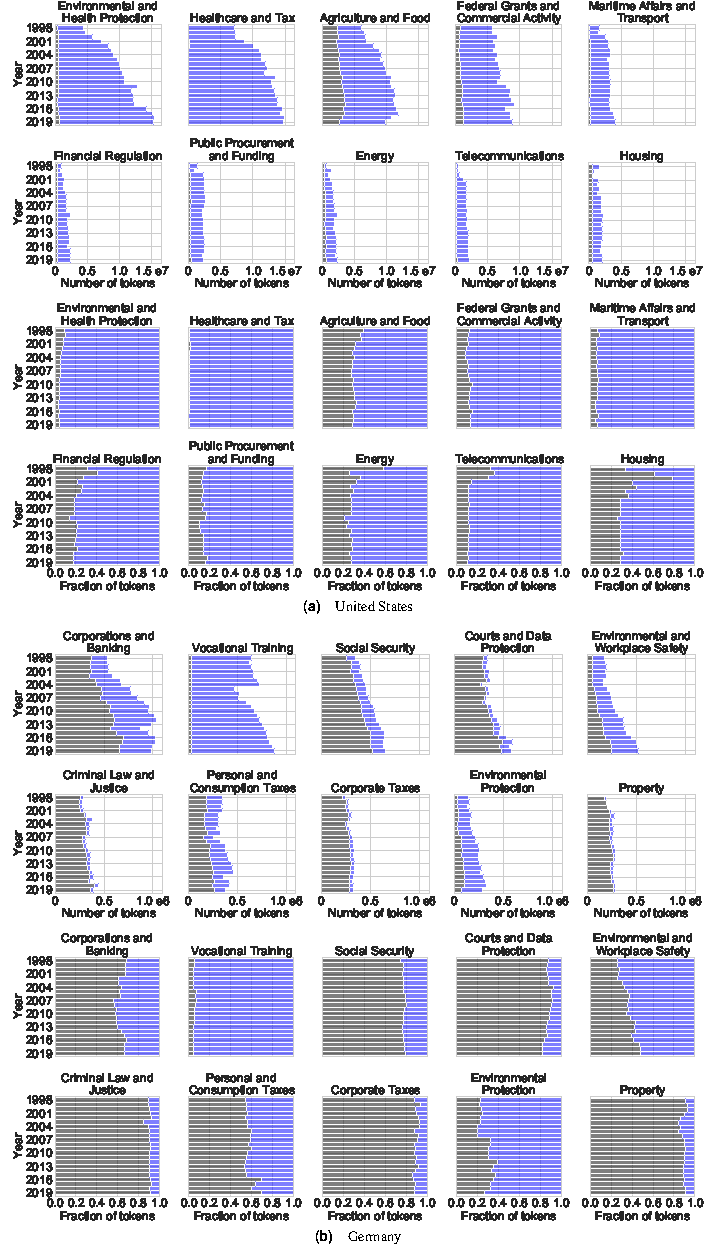
\includegraphics[width=0.75\textwidth]{figure_11}
	\caption{Development of the top ten cluster families from $1998$ to $2019$ as measured by their absolute size in tokens (rows $\{1,2,5,6\}$) and their document type composition (rows $\{3,4,7,8\}$) in the United States (top) and Germany (bottom).
	Black areas represent tokens from statutes and blue areas represent tokens from regulations.}\label{fig:families}
\end{figure}

Inspecting the panels in Figure~\ref{fig:families} in more detail, we observe that the families' ratios of statute tokens to regulation tokens span the whole possible range: 
Some families are \emph{statute-heavy} (i.e., contain mostly statute tokens), 
others are \emph{regulation-heavy} (i.e., contain mostly regulation tokens),
and yet others are \emph{mixed} (i.e., lie between the aforementioned extremes).
For a robust categorization of the ten largest families, the data suggests a threshold of an average $80~\%$ (i.e., an average ratio of $4:1$) over the entire investigation period to classify a family as \emph{x-heavy} for $x\in\{\text{statute}, \text{regulation}\}$.
In the United States, this leads to four mixed families (Agriculture and Food; Financial Regulation; Energy; Housing) and six regulation-heavy families.
In Germany, we find four statute-heavy families (Courts and Data Protection; Criminal Law and Justice; Corporate Taxes; Property), one regulation-heavy family (Vocational Training) and five mixed families.
The overall situation remains similar even if we adopt a simple majority for the classification (eliminating the \emph{mixed} category): 
With the exception of three singular years in two families (Energy in $1998$, and Housing in $1999$ and $2000$), all top families in the United States contain a majority of regulation tokens.
The German data then presents three regulation-heavy families (Vocational Training; Environmental and Workplace Safety; Environmental Protection) and seven statute-heavy families.
A particularly striking example of a statute-heavy family is the Property family in Germany, in which there are nine times as many statute tokens as there are regulation tokens in all years except between $2002$ and $2006$.
The United States cluster family concerning Healthcare and Tax (two topics connected, inter alia, via the tax-based funding of Medicare and Medicaid) represents the opposite extreme, containing almost no statute tokens over the entire period under study.
Interestingly, no family in either country is constantly balanced between statutes and regulations, with the family concerning Personal and Consumption Taxes in Germany coming closest in the period from $1998$ to $2015$.

As Figure~\ref{fig:families} traces the development of the top ten cluster families in each country over time, we can also observe changes in the families' composition.
Extending the terminology adopted above, we can classify the families' growth based on the fraction of growth that is attributable to each of our document types. 
We say that a family is \emph{x-driven} for $x\in \{\text{statute}, \text{regulation}\}$ if tokens from $x$ account for at least $80~\%$ of the family's net growth when comparing $1998$ and $2019$, otherwise, we say that its growth is \emph{mixed}. 
Using these categories, we can classify all of the United States top ten families as regulation-driven
and half of the German top ten families as statute-driven (Social Security; Personal and Consumption Taxes; Criminal Law and Justice; Corporate Taxes; Property), while only one German family is classified as regulation-driven (Vocational Training). 
The full categorization of all top ten families for both countries, both in terms of their average composition and in terms of their growth, can be found in Section~4.3.3 of the~\thesi, 
where we further show that the general tendencies described above also hold for the entire population (although the trends are neither monotone nor universal and their extent differs from family to family).

Overall, the dynamics of the largest cluster families reflect the growth patterns documented in Figure~\ref{fig:basic-statistics}.
In absolute terms, regulations outgrow statutes by large margins in all of the top ten United States families, and statutes moderately outgrow regulations in most of the top ten German families. 
In relative terms, regulations still dominate in the United States, 
and statutes still dominate in Germany (although they are less prominent than they appear when considering absolute numbers).
In summary, based on the top ten families depicted in Figure~\ref{fig:families}, the United States seems to favor rule making via regulations, while Germany seems to favor rule making via statutes, and both countries' preferences appear to get stronger over time.

Finally, to evaluate how federal regulations impact our data-driven map of the United States and German legal systems, we compare the cluster families depicted in Figure~\ref{fig:families} to those derived in prior work that considers only federal statutes \cite{katz2020}.
For the United States, the top ten cluster families based on statutes only have topics similar to those derived from statutes and regulations combined, 
including Environmental and Health Protection, Public Health and Social Welfare, Taxes, Agriculture and Food, Financial Regulation, Public Procurement, Telecommunications, and Federal Grants and Commercial Activity including Small Business Aid.
The topic of Education makes the top ten in the statutes-only data but not in the data containing regulations, while Maritime Affairs and Transport as well as Energy only rise to prominence in the combined data.
In Germany, topics such as Financial Regulation, Taxes, Social Security, Environmental Protection, Criminal Law and Justice, and Property represent sizeable cluster families based on both datasets. 
The topic of Public Servants, Judges, and Soldiers features prominently only in the results excluding regulations, while the families of Vocational Training and of Environmental and Workplace Safety make the top ten only in the combined data.

First and foremost, however, comparing our results to those from \cite{katz2020} demonstrates that adding federal regulations to the data results in a more accurate map of law.
For example, the German data from \cite{katz2020} features a family on Market and Network Regulation that includes a leading cluster on (renewable) energy law, while no comparable family exists in the United States.
Having added federal regulations, we now see such a family in the top ten also in the United States, whose prominent position is explained by its mixed composition (including more than $70~\%$ regulation tokens on average).
At the same time, a cluster concerning (renewable) energy law is now part of the Environmental and Workplace Safety family in Germany because its regulations connect it more closely to rules concerning the protection of the environment than its statutes alone.
This suggests that adding yet further document types, e.g., federal court decisions, to our data will continue to improve the legal maps produced using our methodology, making this a promising avenue for further research.

\vspace*{6pt}
\subsubsection{Micro-level connectivity}
\label{subsubsec:results:connectivity:micro}

We analyze the connectivity of the United States and German legal systems on the micro level in order to identify those code sections that play a particularly important role in mediating the information flow between the sections which they reference and the sections by which they are referenced.
More precisely, we apply the method sketched in Section~\ref{subsec:methods:connectivity} to the graphs induced by the reference edges, where we keep a star if it has at least ten nodes in total. 
We classify these stars (and their hubs) into sinks, hinges, and sources depending on the ratio between their hubs' in-degree and their hubs' out-degree, and hypothesize that hubs of the same type have a similar function within the legal system. 
We explore the merits of this hypothesis by identifying and classifying the stars of each type in $1998$ and $2019$ and analyzing the content of the top five stars (i.e., those with the largest number of nodes) of each type in $2019$ as shown in Table~\ref{tab:structures}.

\begin{table}
	\centering
	% !TeX spellcheck = en_US
\renewcommand{\arraystretch}{1.5}
\renewcommand{\footnotesize}{\fontsize{6.5pt}{8pt}\selectfont}
\footnotesize
	\begin{tabular}{rrrrlp{0.35\textwidth}p{0.35\textwidth}}
\toprule
   $n$ &   $m_S$ &   $\delta^+$ &   $\delta^-$ & \textbf{Type}   & \textbf{Hub}                                                                      & \textbf{Description}   \\
\midrule
  2721 &     933 &            2 &         2719 & Sink            & 5 USC 552 Public information;\newline agency rules, opinions, orders, records, and proceedings                            & Authority to delegate agency rules, records, etc. to regulations                       \\
  \rowcolor{lightgray!30}1702 &      26 &            1 &         1700 & Sink            & 40 CFR 721.125 Recordkeeping requirements                                   & Authority to require particular records to be kept                        \\
  \rowcolor{lightgray!30}1684 &      28 &            3 &         1680 & Sink            & 40 CFR 721.185\newline Limitation or revocation of certain notification requirements& Criteria and procedure for limitation or revocation of notifications by an agency                        \\
  1173 &     298 &            3 &         1171 & Sink            & 5 USC 552a Records maintained on individuals                          & General definitions and procedure for keeping records on individuals                        \\
  \rowcolor{lightgray!30}1023 &      13 &            0 &         1022 & Sink            & 40 CFR 721.80 Industrial, commercial, and consumer activities                & Definition of a new use of a regulated substance                        \\
   283 &      74 &           31 &          254 & Hinge           & 8 USC 1101 Definitions                                          & Definitions for subchapter on immigration and nationality                         \\
   \rowcolor{lightgray!30}218 &     150 &          114 &          213 & Hinge           & 49 CFR 171.7 Reference Material                                              & Collection of materials to be incorporated by reference in other subchapters                       \\
   \rowcolor{lightgray!30}141 &      34 &           34 &          127 & Hinge           & 49 CFR 172.101 Purpose and use of hazardous materials table                  & Collection of substances deemed hazardous materials                       \\
   138 &      18 &           20 &          117 & Hinge           & 10 USC 101 Definitions                                                   & Definitions including bundling of statutes                       \\
   127 &       8 &           24 &          103 & Hinge           & 15 USC 637 Additional Powers                                              & Authority to carry out actions required throughout the chapter                      \\
   \rowcolor{lightgray!30}215 &      23 &          213 &            1 & Source          & 7 CFR 2.22\newline Under Secretary for Marketing and Regulatory Programs            & Enumeration of stand-in duties contained in other statutes                       \\
   \rowcolor{lightgray!30}177 &      13 &          174 &            2 & Source          & 7 CFR 2.21\newline Under Secretary for Research, Education, and Economics            &  Enumeration of stand-in duties contained in other statutes                      \\
   \rowcolor{lightgray!30}150 &      36 &          149 &            0 & Source          & 19 CFR 178.2 Listing of OMB control numbers                                 & Mapping of documents in other parts to control numbers from the Office of Management and Budget                      \\
   \rowcolor{lightgray!30}133 &      16 &          128 &            4 & Source          & 7 CFR 2.16 Under Secretary for Farm Production and Conservation              & Enumeration of stand-in duties contained in other statutes                     \\
   \rowcolor{lightgray!30}129 &       8 &          128 &            0 & Source          & 7 CFR 2.79 Administrator, Agricultural Marketing Service                     & Enumeration of stand-in duties contained in other statutes                          \\
\bottomrule
\end{tabular}
			
{\vspace*{3pt}\small \textbf{\textsf{(a)}}\quad United States}\vspace*{6pt}
	
\begin{tabular}{rrrrlp{0.35\textwidth}p{0.35\textwidth}}
\toprule
   $n$ &   $m_S$ &   $\delta^+$ &   $\delta^-$ & \textbf{Type}   & \textbf{Hub}                                                                            & \textbf{Description}   \\
\midrule
   256 &      19 &            0 &          255 & Sink            & § 36 Gesetz über Ordnungswidrigkeiten                                                   & Determination of the competent authority to prosecute misdemeanor   \\
   224 &       6 &            0 &          223 & Sink            & § 4 Berufsbildungsgesetz                                                                & Authority to delegate vocational training regulations (professions)                      \\
   194 &       0 &            1 &          192 & Sink            & § 25 Gesetz zur Ordnung des Handwerks                                                   & Authority to delegate vocational training regulations (crafts)                        \\
   191 &       3 &            0 &          190 & Sink            & § 1 Berufsbildungsgesetz                                                                & Goal and definitions for vocational training                      \\
   180 &      24 &           16 &          168 & Sink            & § 1 Gesetz über das Kreditwesen                                                         & Definitions for financial and banking regulation                       \\
   131 &      27 &           88 &           46 & Hinge           & § 3 Einkommensteuergesetz                                                               & Enumeration of tax-free income types                       \\
    88 &       0 &           74 &           13 & Hinge           & Art 229 Weitere Überleitungsvorschriften\newline Einführungsgesetz zum Bürgerlichen Gesetzbuche & Transitional provisions of the civil code                       \\
    86 &       1 &           18 &           68 & Hinge           & § 60 Lebensmittel-, Bedarfsgegenstände-\newline und Futtermittelgesetzbuch                      & Misdemeanors in food and feed safety                       \\
    84 &       0 &           73 &           10 & Hinge           & Art 97 Übergangsvorschriften\newline Einführungsgesetz zur Abgabenordnung                       & Transitional provisions of the fiscal code                       \\
    82 &       0 &           61 &           20 & Hinge           & § 100a Strafprozeßordnung                                                               & Definition of particularly serious crimes\newline allowing for telecommunication surveillance                       \\
    \rowcolor{lightgray!30}76 &       0 &           75 &            0 & Source          & § 69a Straßenverkehrs-Zulassungs-Ordnung                                                & Misdemeanors in traffic and road safety                       \\
    73 &       1 &           71 &            2 & Source          & § 340 Kapitalanlagegesetzbuch                                                           & Misdemeanors in the capital investment code                        \\
    59 &       0 &           56 &            2 & Source          & § 194 Gesetz zum Schutz vor der schädlichen Wirkung\newline ionisierender Strahlung             & Misdemeanors in the radiation protection statute                      \\
    \rowcolor{lightgray!30}48 &       0 &           47 &            0 & Source          & § 184 Verordnung zum Schutz vor der schädlichen Wirkung\newline ionisierender Strahlung         & Misdemeanors in the radiation protection regulation                       \\
    48 &       1 &           45 &            3 & Source          & § 120 Gesetz über den Wertpapierhandel                                                  & Misdemeanors and authority to delegate in the securities trading act                       \\
\bottomrule
\end{tabular}



				
{\vspace*{3pt}\small \textbf{\textsf{(b)}}\quad Germany}

	\caption{%
		Top five reference stars of each type in $2019$ for the United States (top) and Germany (bottom), 
		with stars whose hubs are contained in regulations marked grey.
		Edge and degree counts exclude multi-edges; 
		$m_S$ is the number of edges between spokes, 
		$\delta^+$ is the hub's out-degree, 
		and $\delta^-$ is the hub's in-degree.
	}\label{tab:structures}
	\vspace*{-6pt}
\end{table}

In the United States, we find that hubs of the same type indeed play similar roles in the legal system: 
\emph{Sinks} contain delegation of authority and general procedures, e.g., for record keeping, that are relevant for and therefore referenced by many other sections.
\emph{Hinges} connect entire collections, enumerations, and definitions to one another. 
49~CFR~§~171.7 is an example, as its only function is the incorporation of material collections by external parties (such as the American National Standards Institute) into other sections of the CFR like 49~CFR~§~173.306, which itself serves as a hub for other sections. 
\emph{Sources} enumerate duties contained in other statutes (four of the top five stem from the CFR title on Agriculture, in which this drafting technique seems to be popular) or provide a document map for their respective chapter. 

In Germany, the results paint a similar picture:
\emph{Sinks} contain provisions for delegation of legislative authority (as expected by legal theory), competencies, statements of goals, or definitions.
\emph{Hinges} contain transitional provisions, 
which are designed to bridge between old and new rules, as well as definitions.
The definition classified as a hinge (§~100a Strafprozeßordnung) establishes a well-known connection between the Criminal Code and its definition of crimes and investigative methods described both inside and outside the Code of Criminal Procedure.
All \emph{sources} (and one hinge) are collections of misdemeanors to sanction violations of rules contained in their respective statute or regulation, 
and they encompass activities as diverse as road traffic, securities trading, and handling radioactive materials.
Hence, our classification correctly identifies examples of this popular drafting technique.

As suggested in Section~\ref{subsubsec:methods:connectivity:micro} and confirmed for the largest stars, the type of a star contains information about a section's function within the legal system.
Examining the hundred largest stars, whose types are shown in Table~\ref{tab:star-statistics}, exposes different trends in both countries.
In the United States, sinks dominate both across document types and over time, accounting for three out of four stars in $1998$ and six out of seven stars in $2019$, which points to a pronounced drafting preference.
At the local level, sections of the United States codified law are mostly connected (only) by referencing the same section, which often contains a definition or the description of a procedure.
In Germany, the composition is more balanced to begin with, but sinks still make up the largest share in $1998$. 
Over time, though, the number of sinks and sources amongst the hundred largest stars decreases in favor of hinges. 
Hence, individual sections are no longer only connected by a reference to the same section, but the frequently referenced sections themselves increasingly reference other sections.
As a consequence, the number of sections that are reachable from any individual section in two hops (i.e., following two references) increases.
This makes the information flow via references more efficient, which could explain the reduced need for structural elements to guide information flow via hierarchy in Germany when compared to the United States.
But it also increases the prevalence of reference chains, possibly making the German legal system progressively harder to navigate.

\begin{table}
	\centering
	% !TeX spellcheck = en_US
\renewcommand{\arraystretch}{1.5}
\begin{multicols}{2}
	\begin{tabular}{rrrrr}
\toprule&\multicolumn{2}{c}{\textbf{1998}}&\multicolumn{2}{c}{\textbf{2019}}\\
        &   \textbf{S-Hub} &   \textbf{R-Hub} &   \textbf{S-Hub} &   \textbf{R-Hub} \\
\midrule
   \textbf{Sink} &           60 &           16 &           56 &           30 \\
  \textbf{Hinge} &            8 &            1 &            6 &            3 \\
 \textbf{Source} &            0 &           15 &            0 &            5 \\
\bottomrule
\end{tabular}

	{\vspace*{6pt}\small \textbf{\textsf{(a)}}\quad United States}\vspace*{6pt}
	\newpage
	\begin{tabular}{rrrrr}
\toprule&\multicolumn{2}{c}{\textbf{1998}}&\multicolumn{2}{c}{\textbf{2019}}\\
        &   \textbf{S-Hub} &   \textbf{R-Hub} &   \textbf{S-Hub} &   \textbf{R-Hub} \\
\midrule
   \textbf{Sink} &           42 &            0 &           33 &            0 \\
  \textbf{Hinge} &           30 &            0 &           52 &            1 \\
 \textbf{Source} &           17 &           11 &            8 &            6 \\
\bottomrule
\end{tabular}
	
	{\vspace*{6pt}\small \textbf{\textsf{(b)}}\quad Germany}
\end{multicols}

	\caption{%
		Types of the top hundred reference stars (i.e., those with the largest number of nodes) in $1998$ and $2019$ for the United States (left) and Germany (right). S-Hubs are hubs contained in statutes and R-Hubs are hubs contained in regulations.
	}\label{tab:star-statistics}
\end{table}

Mirroring the larger trends described in Section~\ref{subsubsec:results:connectivity:macro} and Section~\ref{subsubsec:results:connectivity:meso}, regulations play a more important role in the United States than in Germany at the micro level of connectivity as well. 
While the total share of regulation hubs in Germany is small, 
they make up almost half of the sources amongst the top hundred reference stars in $2019$, which again follows the larger pattern of regulations referencing rather than being referenced.
In the United States, regulation hubs account for just under $40~\%$ of the top hundred reference stars, 
but almost all of the largest stars are sinks, regardless of the document type of their hub.
This suggests that the United States drafting dynamics resulting in sinks affect both the executive and the legislative branches of government. 

\vspace*{6pt}
\subsection{Profiles}
\label{subsec:results:profiles}

In a step toward developing a dashboard for measuring and monitoring the law, 
we demonstrate the utility of the profiling procedure described in Section~\ref{subsec:methods:profiles} by applying it to selected statutes and regulations from the United States and Germany in a case study focusing on financial regulation. 
We profile a total of four statutes (two from each country) that constitute landmark legislation in this domain and trace their statistics over time in Figure~\ref{fig:profiles}, 
along with those of two additional regulations from the same area.

\begin{figure}
	\centering
	\vspace*{-8pt}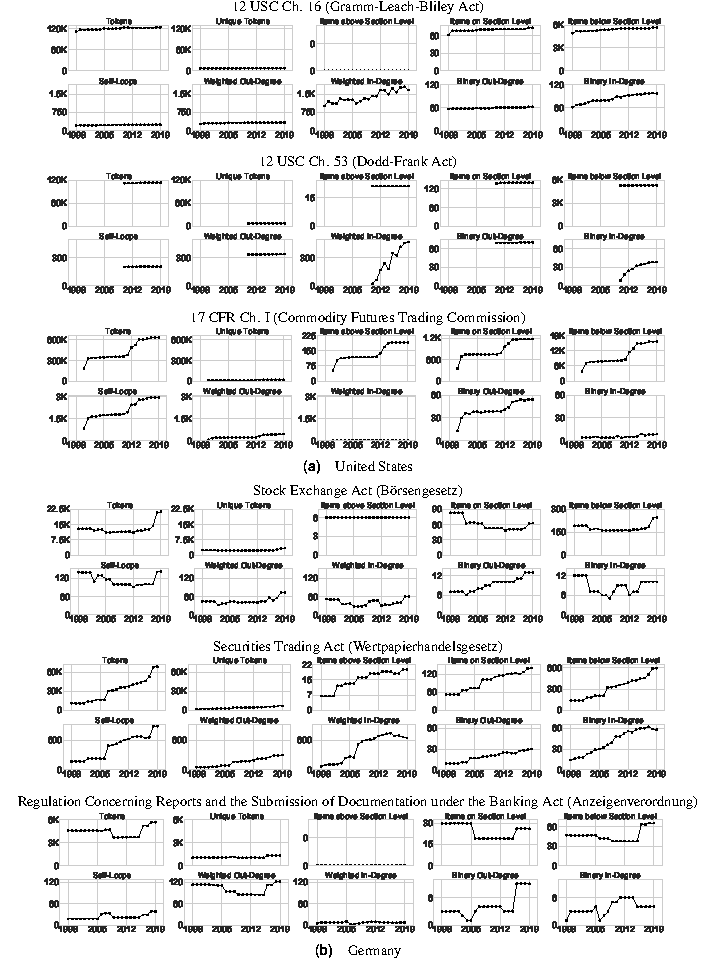
\includegraphics[width=\textwidth]{figure_12}\vspace{-6pt}
	\caption{%
		Profiles tracking the evolution of selected laws related to financial regulation for the United States (top) and Germany (bottom) from $1998$ to $2019$.
	}\label{fig:profiles}
\end{figure}

12~USC~Ch.~16, popularly known as the Gramm-Leach-Bliley Act or Financial Services Modernization Act of 1999 (GLBA), liberalized the United States financial market by allowing the combination of investment banks, commercial banks, and insurance companies in one institution. 
It has been in effect for nearly our entire investigation period ($1999$--$2019$) and, as indicated by nearly flat lines in all but the panels related to in-degree, has not materially changed.
However, the interaction of the GLBA with other parts of the legal system has been anything but static, with its initial weighted in-degree of $1000$ increasing by $60~\%$ between $1999$ and $2019$ due to incoming references from other statutes and regulations.
Unlike the growth trend in the weighted in-degree, the growth trend in the binary in-degree is nearly monotonic. 
This indicates that most of the fluctuations in the GLBA's regulatory environment occur within individual chapters of the USC or the CFR.
In summary, the GLBA can therefore be rightfully regarded as a landmark statute, which has required little engineering but has remained an important reference throughout the period under study.

The profile of 12~USC~Ch.~53, popularly known as the Dodd-Frank Act or the Wall Street Reform and Consumer Protection Act (DFA), shows similarities with the GLBA in most statistics we track.
Introduced in response to the Great Recession in $2010$, 
it is approximately half as old as the GLBA, 
and like the GLBA, it has barely changed in size, breadth, or structure.
But although the DFA is comparable to the GLBA in size, 
its interaction with the environment seems much more dynamic, 
with its weighted in-degree increasing by a factor of almost ten over its lifetime.
In absolute terms, however, the references increase by less than $500$, i.e., in the same order of magnitude as for the GLBA.
This is in line with the fact that both statutes are part of the same legal domain, and it highlights how much the evolution of individual pieces of legislation is influenced by their initial conditions, e.g., whether they are strongly connected with their environment already at birth.
For the DFA, the growth of the weighted in-degree again is not monotonic, 
but it is visibly steeper before $2017$ than afterwards, leveling off in the last years of the period under study.
The binary in-degree, whose gradient is almost monotonically decreasing from the start, anticipates this deceleration by several years.
This suggests the existence of an onboarding period, in which the DFA is integrated into the regulatory environment before finding its place in the United States legal system (see the related discussion in \cite{mclaughlin2021}).

The profiles of the two German statutes we examine are starkly different from those of the United States statutes.
Statutes under the names of both the Stock Exchange Act (SEA) and the Securities Trading Act (STA) have been in effect for the entire observation period.
As indicated by their unique token count, they are both constantly narrow in thematic scope (with the STA an order of magnitude more narrow than the SEA to start with), 
and their token count increases over time.
While the SEA and the STA start at comparable sizes in $1998$, the STA grows by a factor of seven, while the SEA merely doubles.
Possibly as a result, the SEA largely maintains its original number of structures,
while the number of structural elements in the STA triples.
This is accompanied by an expected, nearly parallel increase in the number of STA sections, 
and even a decrease of about $25~\%$ in the number of SEA sections.
Beyond the general growth trends present in almost all STA statistics,
the period from $2006$ to $2007$ stands out, as most of its statistics experience a relatively steep increase between these years.
The doctrinal investigation prompted by this observation reveals that the source of the increases is a legislative project translating extensive transparency requirements mandated by the European Union into German law (Transparenzrichtlinie-Umsetzungsgesetz), which came into effect in January $2007$.
This finding also shows how our methods can complement doctrinal legal scholarship, as has been demonstrated, e.g., for the development of the STA over its entire lifetime \cite{coupette2019a}.

Our statistics produce interesting insights not only for statutes but also for regulations.
For example, there is a noticeable increase in the self-referentiality of the CFR chapter about the Commodity Futures Trading Commission (CFTCR),
and the German Reports and Documents Regulation (RDR) shows structural changes between $2005$ and $2006$ as well as between $2015$ and $2016$.
As our framework enables the joint modeling of data from different document types, its application can surface characteristic differences between these types, too.
Examining our exemplary regulations and statutes in Figure~\ref{fig:profiles},
we find that the CFTCR experiences noticeable growth (about $200~\%$),
while the size of the featured statutes barely changes.
At the same time, the regulation's weighted in-degree is several orders of magnitude smaller than that of the DFA or the GLBA, supporting the intuition that statutes should be referenced more frequently than regulations for this particular case. 
In Germany, the RDR is smaller than the featured German statutes,
and it covers less diverse content (as would be expected for a regulation from a legal theory perspective).
Its structural organization is minimal, as is its self-referentiality.
This confirms that smaller units of law require less internal organization by both structure and references.
The RDR references, and is referenced by, a small number of different documents, indicating homogeneity in its regulatory environment.
Its weighted out-degree falls between the SEA and STA, i.e., it has a non-negligible number of references to a limited number of targets.
In summary, the RDR has most characteristics expected from a German regulation, and its overall profile can clearly be distinguished from that of the featured German statutes.

Our framework enables comparisons not only across document types but also across countries.
When examining the DFA and the STA, we see that the STA starts at a size of roughly a third of the DFA but grows to two thirds of the DFA over time.
Both statutes have similar degrees of structure at the section level and above,
but the DFA contains ten to fifteen times the amount of items below section level, indicating a vastly more granular hierarchical organization.
Conversely, the STA contains three to four times more self-loops than the DFA, with its weighted in-degree about $1.5$ times and its binary in-degree between $1.5$ and $2$ times higher than those of the DFA after the first couple of years.
This mirrors the more general finding that rule-making agents in the United States and Germany favor different mechanisms to handle the token growth of their statutory corpora: 
Americans like adding hierarchical structure, while Germans prefer adding references \cite{katz2020}.

Figure~\ref{fig:profile-graphs} combines profile statistics concerning size and interdependence to enable direct visual comparisons. 
Here, we compare the ego graphs of the DFA and the STA for every quarter of their existence during our investigation period.
Note that the distance between the snapshots is different for both statutes, 
as the DFA was adopted only in the middle of our study period, but both series end in $2019$.
Complementing the statistics presented in Figure~\ref{fig:profiles}, the visualization attributes the references to their actual sources and targets, indicating their number by the weight of the edges.
For the DFA, its \emph{reliance} (i.e., how much and how diversely it references other statutes and regulations) barely changes,
while its \emph{responsibility} (i.e., how much and how diversely it is referenced by other statutes and regulations) discernibly increases, 
as the DFA becomes more and more integrated with its environment.
In contrast, both the reliance and the responsibility of the STA increase over time, with its responsibility starting nearly twice as high and increasing at a much faster rate than its reliance.
As shown by the edge colors, the diverse responsibility of the STA concerns both statutes and regulations,
and the DFA is most intensively responsible for regulations.
In line with the expectation derived from legal theory,
both the DFA and the STA rely mostly on statutes.

\begin{figure} 
	\centering
	\vspace*{-8pt}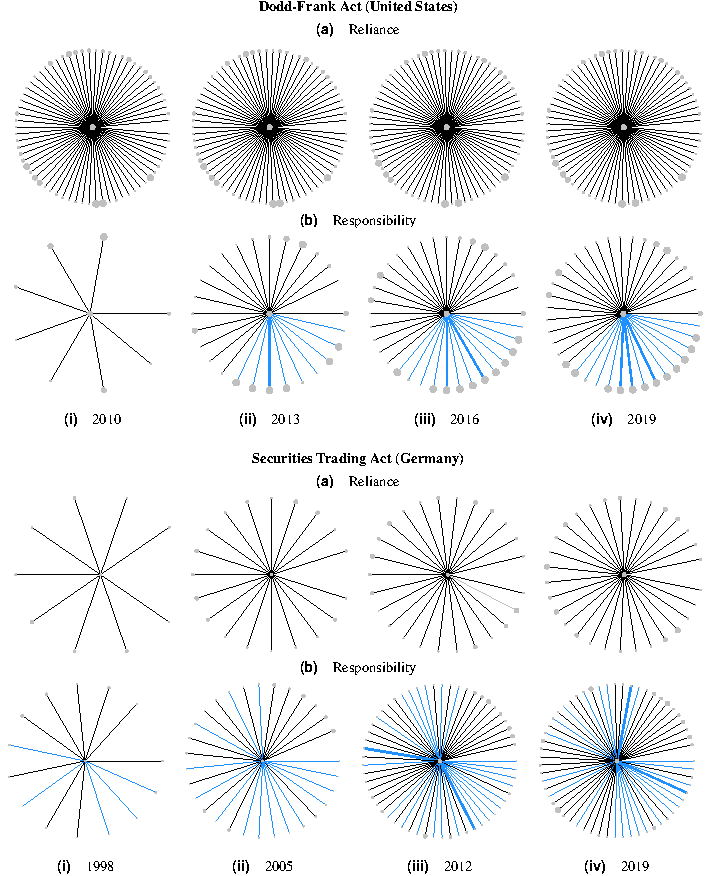
\includegraphics[width=\textwidth]{figure_13}
	\caption{Reliance and responsibility of the Dodd-Frank Act (DFA, top) and the Securities Trading Act (STA, Wertpapierhandelsgesetz, bottom) from $1998$ to $2019$.
	Leaf nodes are chapters of the USC or the CFR that are cited by (reliance) or cite (responsibility) the DFA (top), 
	and statutes or regulations (or their books, if applicable) that are cited by (reliance) or cite (responsibility) the STA (bottom).
	Edge types indicate reference types as used in Figure~\ref{fig:crossref-differentiation} (black for lateral statute references, light blue for upward references, and silver for downward references).
	Node size is proportional to the node's number of tokens;
	edge width is proportional to the number of references represented by the edge.
	}\label{fig:profile-graphs}
\end{figure}
